With $\kappa=12$ knobs and the standard CMA-ES population size $\lambda=11=4+\lfloor3.log(\kappa)\rfloor$, the algorithm usually lasts less than $2000\ BeATS\ evaluations$ (i.e. $180\ generations$) to converge, which is  approximately 3 hours on a regular computer without parallelization.
$U^{global}$ is set to a reasonable $5\%$, in order to give some space to CMA-ES on the global quantities.\\
Denoting $\widetilde{F}$ the average over $i\in T$ of $\widetilde{F_{i}}$, we define $U^{add}$, the mainline sensor confidence interval uncertainty, as a percentage of $\widetilde{F}$. For example, $\frac{U^{add}}{\widetilde{F}}=5\% \Rightarrow U^{add}=5139\ cars$.
The main observation, that we will develop later, is that the templates shape limit the quality of the result : in every experiment, not one but two congestion profiles appear on the contour domain and are correlated (i.e. when one grows, the other one too : they are caused by the same knobs).  $\mathscr{C}$ matching the unique box $\widetilde{\mathscr{C}}$ implies that the undesirable congestion profile is significant and outside the box.\\
We will judge the quality of the results of an experiment by the value of $J^{*}$ \emph{and} the likelyhood of the shape of the congested domain $\mathscr{C}$. \\
It is important to highlight that, for a given set of parameters, even tough the result quality is equivalent from one algorithm execution to another, the solution input $k^{*}$ found are very different. The solution of our calibration process is far from being unique for this experiment.\\
We will therefore say abusively that there are several "equivalent global minima" for J.
\\
\emph{Changing the parameters:}\\
Fig. \ref{fig:results_array}. below contains the parameters and global error results of the experiments we made. We monitored the effect of each parameter by changing it slightly from one execution to another. Going in the details of each execution, we will expose in the following sub-sections the effect of these parameters on the result quality. The exact values of the parameters in our case are not relevant as they depend on the scenario, time, sensor distribution, and data quality : this study is only qualitative. 
\begin{figure}
\centering
	\caption{Experiments parameters and $J$ final value.}
	\label{fig:results_array}
	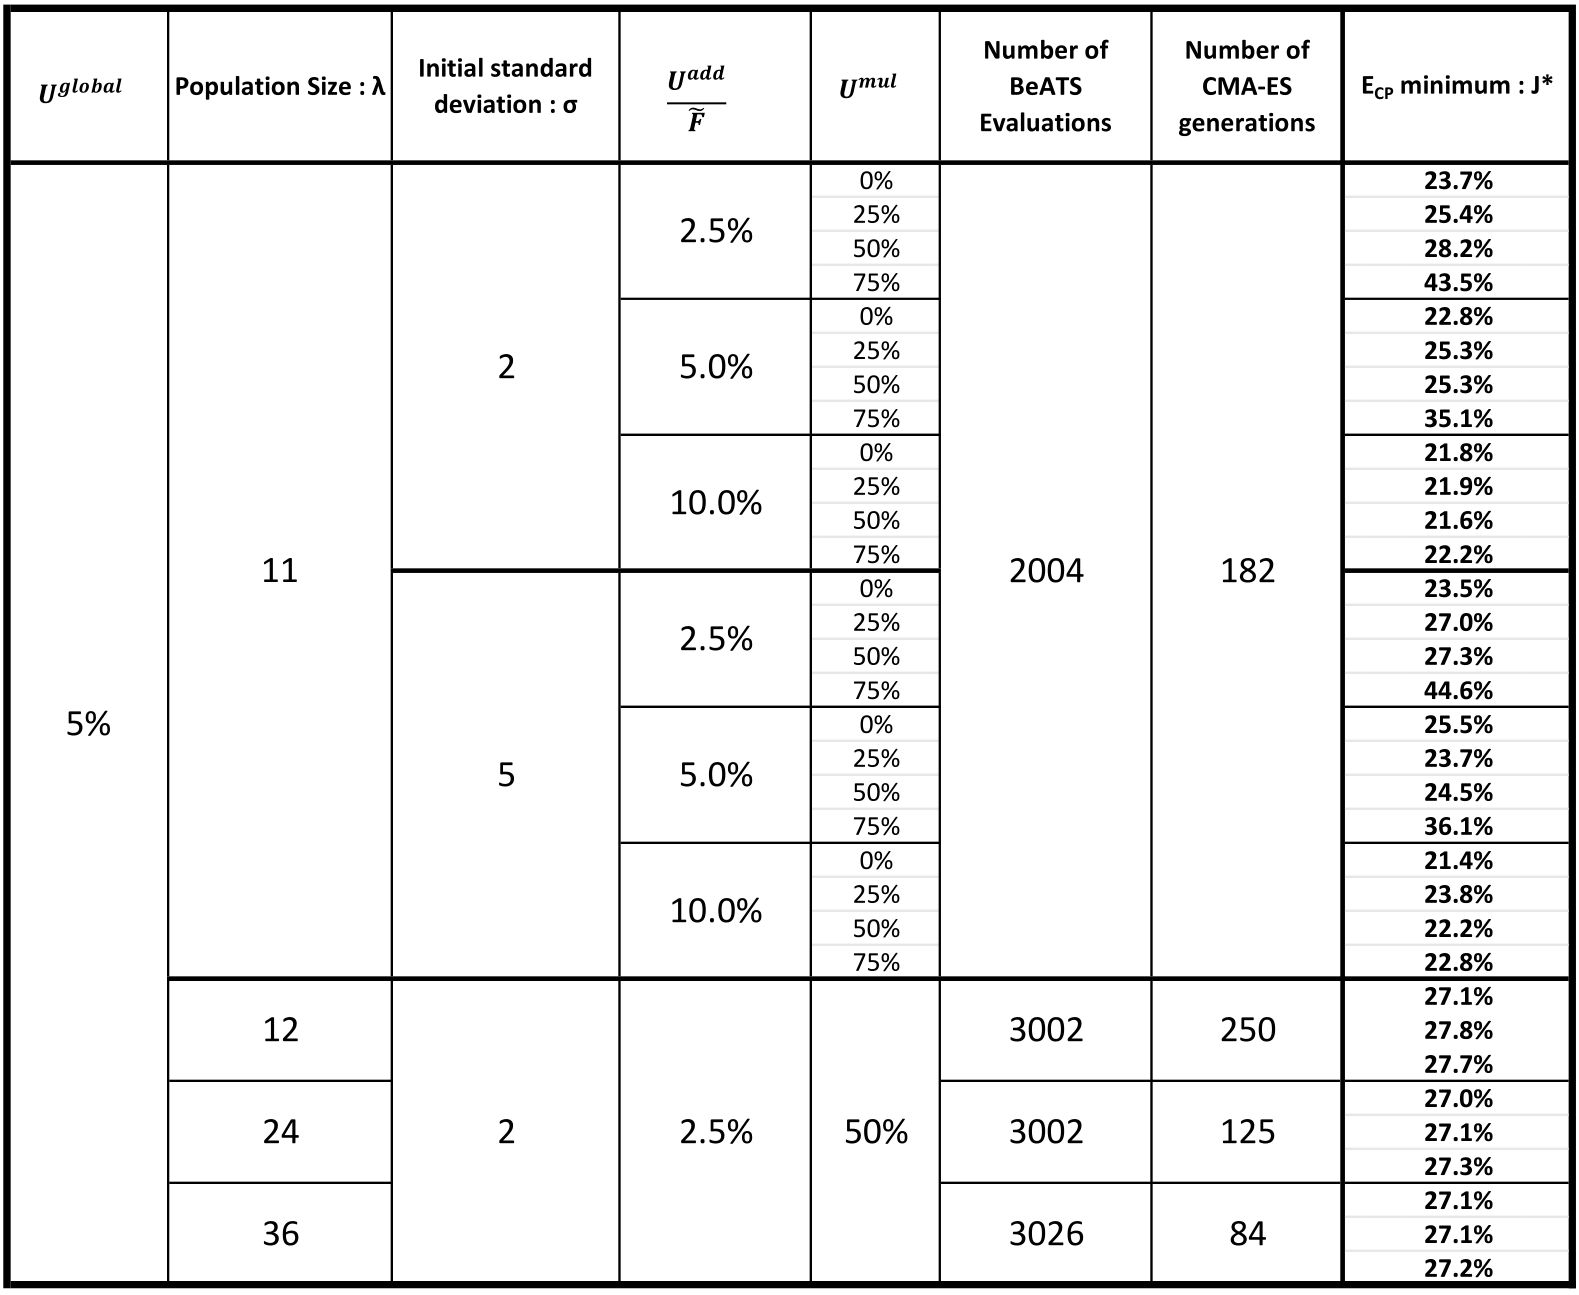
\includegraphics[width=7in]{figures/results_array.png}
\end{figure}
\newpage


